\newcommand{\titreA}{Rapport de projet}
\newcommand{\titreB}{Projet industriel}
\documentclass[12pt]{article}
\usepackage[utf8]{inputenc}
\usepackage[francais]{babel}
\usepackage[T1]{fontenc}
\usepackage{lmodern, marvosym, geometry, graphicx, multicol, lastpage, tikz, listings}
\usepackage[hyperindex=true, colorlinks=true, breaklinks=true, linkcolor=blue]{hyperref}
\usepackage{fancyhdr, verbatim, alltt, pdfpages}

\geometry{hmargin=1.5cm, vmargin=2cm}
\addtolength{\parskip}{10pt}
\pagestyle{fancy}

\definecolor{lightgray}{gray}{0.9}
\definecolor{darkgray}{gray}{0.4}
\newcommand{\hlc}[1]{\color{purple}{\textbf{#1}}}
\lstset{language=,
    basicstyle=\sffamily\footnotesize,
    xleftmargin=20pt,
    xrightmargin=20pt,
    numbers=left,
    stepnumber=1, % le pas des numeros de ligne
    numbersep=10pt,
    breaklines=true,
    tabsize=4,
    %frame=single,
    showspaces=false,
    showstringspaces=false
    inputencoding=utf8, %put1 d'utf8 dans listing
    extendedchars=true, %put1 d'utf8 dans listing
    literate={à}{{\`a}}1 {é}{{\'e}}1 {è}{{\`e}}1 {ê}{{\^e}}1 {â}{{\^a}}1 {î}{{\^i}}1 {ê}{{\^e}}1 {É}{{\'E}}1 {À}{{\`A}}1 {«}{{\og}}1 {»}{{\fg{}}}1 {ô}{{\^o}}1 {ù}{{\`u}}1 {û}{{\^u}}1 {ç}{{\c{c}}}1 {Ç}{{\c{C}}}1 {--}{{-\,-}}1 {-}{{-}}1 {*}{{*}}1 {Switch(config)\#}{{\textbf{Switch(config)\# }}}1 {Switch(config-if)\#}{{\textbf{Switch(config-if)\# }}}1 {Switch(config-line)\#}{{\textbf{Switch(config-line)\# }}}1 {Switch>}{{\textbf{Switch> }}}1 {Switch\#}{{\textbf{Switch\# }}}1, %put1 d'utf8 dans listing
    columns=fullflexible, % suppression des espaces autour des deux-points
    escapechar=§, % permet d'insérer du §code latex§
    backgroundcolor=\color{lightgray},
    alsoletter={.,1,2,3,4,5,6,7,8,9,0},
    keywords={path_to_certs, user_login, user_password, nom_entreprise, pass_radius_sql, utilisateur1, pass_utilisateur1, secret_radius, 192.168.1.2, 192.168.1.10, 255.255.255.0, fastethernet0/1, vlan_id, pass_enable, pass_enable_secours, utilisateur_secours, pass_utilisateur_secours, pass_root_sql, snack, 192.168.0.254, commutateur1, client1, Nancy, BHConsulting, France, FR, nom_serveur_radius, dossier_certs, dossier_certs_utilisateur, eth0 },
    keywordstyle=\hlc,
    morecomment=[l]{\#}, % commentaires shell en ligne
    commentstyle=\itshape\color{darkgray},
}

\renewcommand{\headrulewidth}{1pt}
\lhead{\textbf{\titreA{} (\titreB)}}
\rhead{\emph{BOUGET / GUÉPIN / PINHÈDE / VAUBOURG}}
\lfoot{TELECOM Nancy - PI}
\cfoot{\thepage{} / \pageref{LastPage}}
\rfoot{2012-2013}

\begin{document}
\thispagestyle{empty}

\begin{multicols}{2}
{\large
	\begin{flushleft}
		\noindent{}\textbf{Nicolas BOUGET}\\
		\Letter~nicolas.bouget@esial.net\\
		3A TRS1\\~

		\noindent{}\textbf{Julien GUÉPIN}\\
		\Letter~julien.guepin@esial.net\\
		3A IL\\
	\end{flushleft}

	\begin{flushright}
		\noindent{}\textbf{Marc PINHÈDE}\\
		\Letter~marc.pinhede@esial.net\\
		3A LE\\~

		\noindent{}\textbf{Julien VAUBOURG}\\
		\Letter~julien@vaubourg.com\\
		3A TRS2\\
	\end{flushright}
}
\end{multicols}

\vspace{0.5cm}

\begin{center}
	{\Huge\textbf{\titreA}}

	\vspace{1cm}

	{\huge\emph{\titreB}}

	\vspace{1cm}

	\begin{flushleft}
		{\large
		\hspace{3.2cm}
		\textbf{Société~:} B.H. Consulting\\
		\hspace{3.2cm}
		\textbf{Intervenant industriel~:} Guillaume ROCHE\\
		\hspace{3.2cm}
		\textbf{Intervenant universitaire~:} Jean-François SCHEID
		}
	\end{flushleft}

	\vspace{1cm}
	{\large Le \today}

	\vspace{1.5cm}

	
\includegraphics[width=140pt]{img/BHConsulting.jpg}

	\vspace{1.5cm}

	
\includegraphics[width=190pt]{img/ul.png}
	\hspace{3.5cm}
	
\includegraphics[width=140pt]{img/telecom-nancy.jpg}
\end{center}
\newpage

\thispagestyle{empty}
\tableofcontents
\newpage



\listoffigures
\newpage

\section{Introduction}
\subsection{Préambule}

La réalisation du travail décrit dans ce document s'incrit dans une démarche étudiante, visant à valider la dernière année de la formation ingénieure de l'école TELECOM Nancy. Elle s'effectue sur une durée de six mois, en partenariat avec l'entreprise B.H. Consulting. Jean-François SCHEID, maître de conférences et enseignant à l'école, a accepté d'encadrer le projet en tant qu'intervenant universitaire.

L'entreprise rémunère l'école pour le travail effectué en deux paiements, dont le second dépend de sa satisfaction à la vue du travail effectué. L'équipe du projet est constituée de quatre étudiants, qui s'engagent à travailler 1000 heures, soit 250 heures par personne.

Un rapport et une soutenance sont présentés à mi-parcours du projet, pour un rendu final en fin d'année scolaire.

\subsection{TELECOM Nancy}

TELECOM Nancy, école associée de l'Institut Mines-Télécom, est une école d'ingénieurs publique de l'Université de Lorraine. Il s'agit d'une école généraliste en informatique, sciences et technologies du numérique, habilitée par la Commission des Titres d'Ingénieurs (CTI). Elle fait partie du Concours TELECOM INT, et a changé de nom au début de l'année 2012, se faisant connaître jusqu'alors sous le nom de ESIAL.

En plus d'un tronc commun, elle dispose de quatre spécialisations différentes, qui vise quatre domaines distincts~:

\begin{description}
\item[Ingénierie du Logiciel~:] Développement d'applications sûres et robustes, avec un attachement particulier pour le domaine du web.
\item[Logiciels Embarqués~:] Étude des systèmes embarqués et programmation efficace dans des environnements restreints.
\item[Systèmes d'Information d'Entreprise~:] Étude des systèmes d'information et des bases de données.
\item[Télécommunications, Réseaux et Services~:] Étude du fonctionnement et de la gestion des réseaux informatiques.
\end{description}

\subsection{B.H. Consulting}

Initialement crée par Bertrand PÉTAT (gérant actuel) en 2000 dans la région luxembourgeoise, B.H. Consulting s'est importée en France dès 2001. Située à Nancy, l'entreprise est restée en contact avec beaucoup de clients luxembourgeois et continue donc d'assurer ses prestations au Luxembourg, comme en France.

Elle comprend cinq employés~:

\begin{itemize}
\item Bertrand PÉTAT (gérant)
\item Christine MARCILLAT (secrétaire de direction)
\item Guillaume ROCHE (ingénieur réseaux)
\item Jérémy KRAEMER (ingénieur réseaux)
\item Simon KOSMERL (ingénieur réseaux)
\end{itemize}

L'organigramme est disponible en figure~\ref{organigramme} page~\pageref{organigramme}.

\begin{figure}[!h]
	\begin{center}
		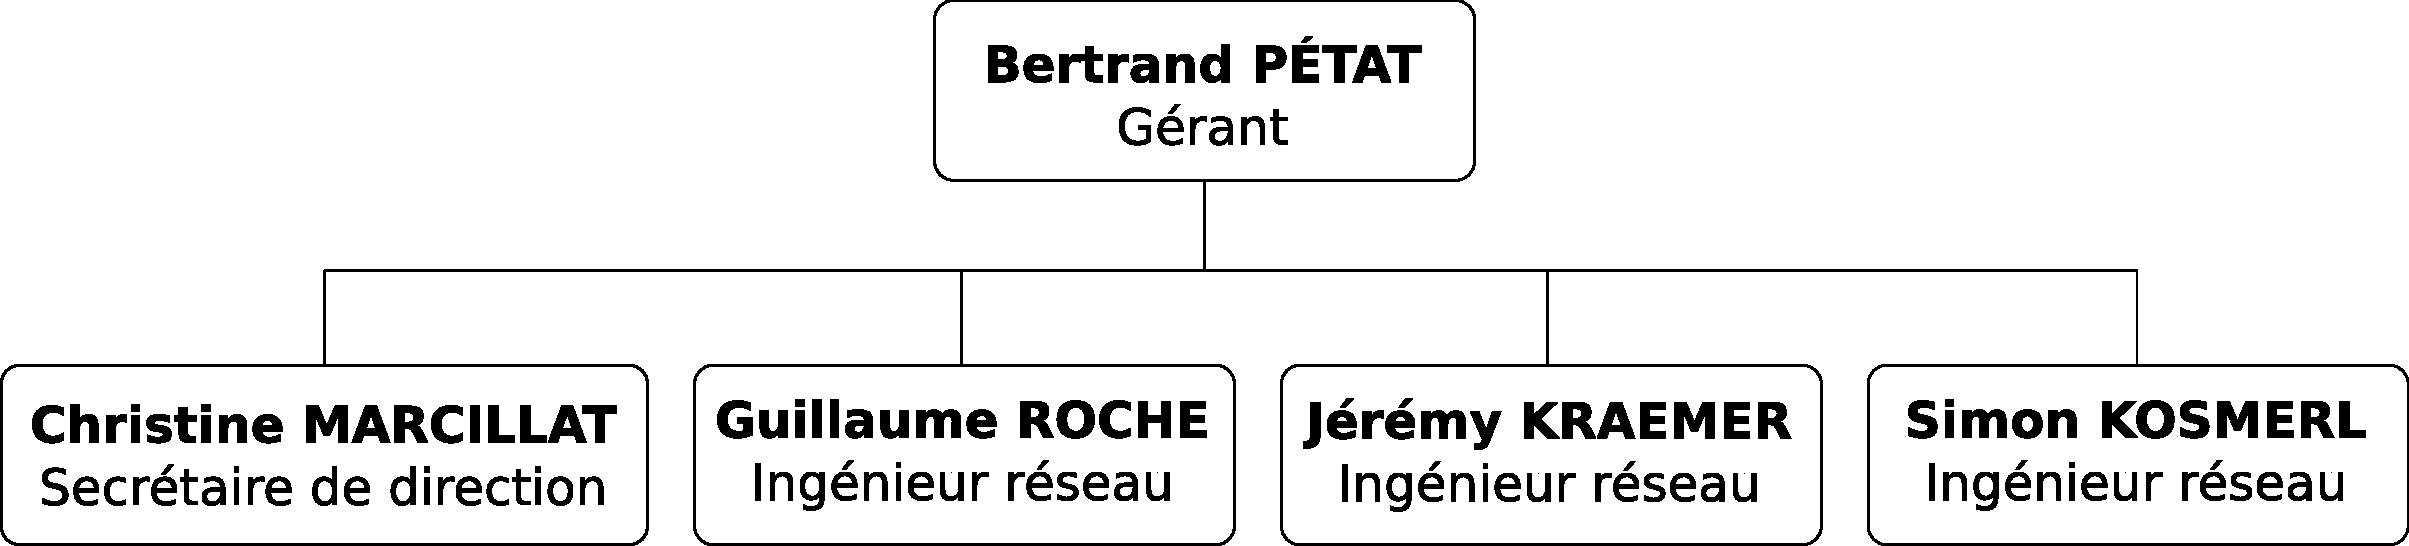
\includegraphics[width=\textwidth]{img/organigramme.pdf}
	\end{center}
	\caption{Organigramme de B.H. Consulting}
	\label{organigramme}
\end{figure}

B.H. Consulting est spécialisée dans les services d'intégration réseau pour les entreprises. Aux côtés de partenaires comme Cisco (équipements réseaux) et Astaro (sécurité), elle conseille et assure l'élaboration d'architectures réseau dans les domaines de l'informatique, de la téléphonie et de la vidéosurveillance. Elle propose des prestations pour des réseaux locaux \og~sur mesure\fg{} selon les attentes du client (adresses IP, sécurité, fiabilité, qualité de service, évolutivité, etc.).

L’entreprise offre un service global qui va de l’étude de cas jusqu’à la mise en oeuvre du réseau et sa maintenance.

Elle propose les prestations suivantes~:

\begin{description}
\item[Proposition de solution~:] Tests et validation des configurations au préalable sur maquette, exposition du choix à l’utilisateur final et décision d’un plan de migration d’architecture.
\item[Mise en oeuvre~:] Configuration, installation et câblage avec le minimum de gêne et de temps d’interruption pour l’activité de l’entreprise.
\item[Analyse fonctionnelle~:] Étude des besoins et des fonctions souhaitées par l’utilisateur compte tenu de son activité, détermination des solutions possibles.
\item[Audit visuel du réseau existant~:] Inventaire informatique, mise en évidence des défauts de câblages, des failles de sécurité ou de fiabilité, des problèmes techniques (alimentation électrique, ventilation), etc.
\item[Maintenance~:] Résolution des différents problèmes rencontrés par l’utilisateur au cours de l’exploitation.
\end{description}

\section{Projet}
\subsection{Contexte}

La sensibilisation croissante aux notions de sécurisation des réseaux des entreprises a conduit B.H. Consulting à devoir répondre à de nouveaux types d'exigences.

Les réseaux d'une entreprise sont en effet devenus un point critique de toutes les nouvelles sociétés, qui sont régulièrement amenées à perdre des heures considérables de travail dès lors que ceux-ci ne sont plus accessibles. Au-delà de l'aspect fonctionnel, les réseaux sont la voie royale vers les serveurs les plus sensibles des administrations, qui y stockent les informations les plus confidentielles.

Qu'ils soient filaires ou non, ces réseaux sont accessibles dès lors qu'on est dans les locaux des entreprises~: prises murales, émissions wifi, etc. N'importe quel individu ayant alors la possibilité de se relier physiquement aux réseaux, il faut mettre en place un mécanisme de contrôle logique pour restreindre ses accès. Pour autant, ce mécanisme ne doit pas être lourd à administrer, ce qui impliquerait rapidement un laxisme et une confusion dans les règles établies. Définir strictement les autorisations en fonction des points d'accès physiques, pour ensuite établir une carte des autorisations de l'ensemble des bâtiments n'est pas non plus la bonne solution, puisqu'il sera difficile de garantir les contrôles d'accès à ces prises. L'utilisation du réseau dépendra également de l'emplacement géographique de l'utilisateur, à l'encontre de toute logique vis-à-vis de la tendance actuelle au nomadisme constaté dans les entreprises.

Pour répondre à toutes ces exigences, critiques pour une entreprise qui souhaite garantir l'intégrité de son réseau et la confidentialité de ses données (tout en sauvegardant la liberté de mouvement de ses employés), B.H. Consulting est régulièrement contraint d'exploiter les nouvelles technologies les plus adéquates. La première problématique de ce projet industriel sera donc de permettre à B.H. Consulting d'avoir à disposition la documentation nécessaire pour déployer l'une des solutions existantes, facilement et rapidement.

Au delà du déploiement, B.H. Consulting souhaite offrir une souplesse d'administration exemplaire de son système, en permettant aussi bien à ses clients que ses propres employés de modifier les permissions des réseaux. Aucune des solutions d'interface existantes ne répondant à ce besoin actuellement, il s'agit du second objectif de ce projet industriel. L'interface devra devra donc être accessible, ergonomique et complète. Des fonctionnalités d'administration poussées comme la gestion d'un historique, d'une console virtuelle et la gestion des équipements actifs la compléteront durant ce projet.

Les objectifs de ce projet industriel émanent directement des besoins des clients, auxquels B.H. Consulting doit faire face.

\subsection{Objectifs}

Plusieurs objectifs peuvent être tirés des problématiques sus-évoquées~:

\begin{enumerate}
\item Définir la technologie qui permettra de définir des accès aux réseaux de façon dynamique, souple et sécurisée.
\item Former l'équipe du projet industriel sur cette technologie, à l'aide de documentations et d'expérimentations concrètes sur les différents aspects sous-jacents.
\item Écrire une documentation sur le sujet qui sera restreinte et utile à B.H. Consulting dans le cadre de ses besoins.
\item Concevoir une solution logicielle permettant le déploiement rapide et efficace de la technologie sur les réseaux des clients.
\end{enumerate}

Une seconde liste d'objectifs se dégage rapidement, de façon relativement indépendante de la première~:

\begin{enumerate}
\item Concevoir une interface permettant la configuration des accès au réseau, avec des profils d'utilisateurs définis par des ensembles de permissions.
\item Ajouter des fonctionnalités supplémentaires à l'interface, comme la console virtuelle, la possibilité de disposer d'un historique des configurations ou la gestion des équipements actifs.
\item Intégrer l'interface dans la solution logicielle proposée lors de la première étape, pour le déploiement de la solution chez les clients.
\end{enumerate}

Afin de répondre aux attentes de l'entreprise de façon optimale, en ayant l'assurance d'être exhaustif et de soulever toute ambiguïté, les objectifs ont nécessité d'être contractualisés. Les documents qui en résultent ont été rédigés en partenariat avec les responsables de l'entreprise, en respectant les étapes classiques d'une gestion de projet.

\section{Gestion de projet}
\subsection{Constitution de l'équipe}

L'équipe du projet est constituée exclusivement d'élèves-ingénieurs de l'école TELECOM Nancy, en dernière année de formation. Après avoir remporté la confiance de l'entreprise pour se faire attribuer ce travail, le chef de projet a confirmé l'équipe suivante~:

\begin{description}
\item[Nicolas BOUGET] Ayant intégré la spécialisation \textit{Télécommunications, Réseaux et Services} (TRS) dès la seconde moitié de la deuxième année de son cursus ingénieur, Nicolas a une sensibilité particulière pour le réseau et l'administration de services. Avec une expérience forte de conception de tests pour un simulateur d'avion, acquise durant son stage de deuxième année, Nicolas dispose d'une rigueur et d'une méthodologie reconnues, avec une sensibilisation aux problématiques du développement de gros projets. Co-responsable du parc informatique de la convention de culture japonaise Anim'Est lors de sa dernière édition, il est également capable de gérer des infrastructures imposantes en supportant un stress important et une nécessité de qualité de service exemplaire. C'est donc naturellement qu'il a été désigné comme chef de projet, dans le cadre de ce travail.\\
\item[Julien GUÉPIN] Julien a choisi la spécialisation \textit{Ingénierie du Logiciel} (IL) lors de sa seconde année à TELECOM Nancy. Véritable passionné de développement web, Julien apporte des compétences extrêmement fortes dans un projet qui nécessite une expertise sérieuse pour aboutir à une solution logicielle munie d'une interface web fonctionnelle, ergonomique et efficace. Avec de nombreuses expériences dans le domaine, il a été capable de prouver ses capacités de nombreuses fois dans le passé, autant au travers de ses stages que ses projets personnels. Actif associativement, Julien s'est notamment investi dans un projet humanitaire au Pérou, développant ainsi des capacités évidentes de travail en équipe et d'organisation personnelle pour conduire un projet complexe vers une réussite reconnue. Particulièrement intéressé par la seconde partie du projet, il est un élément clé de sa réussite.\\
\item[Marc PINHÈDE] C'est une troisième spécialité offerte par l'école que Marc propose en intégrant l'équipe, puisqu'il a choisi dès l'année dernière l'option \textit{Logiciels Embarqués} (LE). Sa passion pour le domaine, ainsi que la rigueur imposée par les environnements embarqués font de lui une ressource particulièrement minutieuse et attachée à la perfection, qui conduit à la performance et l'excellence. Marc a notamment eu l'occasion de prouver ses compétences lors de son stage de seconde année dans un centre de recherche, en y implémentant un compilateur. Avec des capacités d'intégration et de travail en équipe reconnues à chacune de ses implications dans la convention Anim'Est, Marc est un membre essentiel de l'équipe, qui saura mettre à profit ses compétences dans les domaines couverts par ce projet, qui l'intéressent tout autant.\\
\item[Julien VAUBOURG] Également issu de la spécialisation TRS, Julien est un passionné des réseaux qui dispose en plus d'une forte expérience dans le développement. Une double-compétence qu'il a su prouver à plusieurs reprises au travers de ses nombreux stages et projets personnels. Particulièrement impliqué associativement, notamment dans l'administration d'un fournisseur d'accès à Internet participatif, Julien a l'occasion d'intégrer très régulièrement des équipes, tout en étant force de proposition. Également acteur de la dernière édition de la convention Anim'Est auprès de Nicolas et Marc, il intègre naturellement l'équipe avec une capacité de vision d'ensemble du projet.
\end{description}

Il s'agit donc d'une équipe particulièrement pluridisciplinaire, qui saura composer avec ses membres pour aggréger les compétences de chacun afin d'obtenir le meilleur d'eux-mêmes. Tous les membres ayant déjà eu l'occasion de travailler ensemble, l'équipe est dynamique et a été prête à travailler dès le lancement du projet.

\subsection{Note de cadrage}

Suite à une première réunion avec Guillaume ROCHE (intervenant industriel) la note de cadrage a été rédigée. L'objectif de cette note de cadrage était de fournir une base qui nous a permis de discuter ensemble des objectifs et contraintes du projet, de façon plus contractuelle qu'une simple conversation informelle.

Après avoir échangé sur cette base de travail, nous sommes arrivés à une note de cadrage satisfaisant l'encadrant et l'équipe du projet.

La note de cadrage rappelle la problématique et les bénéfices du projet pour l'entreprise, avec un effort de vulgarisation particulier pour la rendre accessible à un non-technicien. Elle détaille précisément le fonctionnement de la technologie retenue en accord avec l'intervenant, et l'objectif de son utilisation pour l'entreprise. 

Un contexte est ensuite proposé, en rappelant le statut particulier du projet industriel et les enjeux qui sont propres aux membres de l'équipe. Le délai ainsi que l'absence de budget sont évoqués, avec le matériel qui est mis à disposition au lancement du projet.

Les objectifs sont complétés par un chapitre sur le niveau de qualité attendu, avec une priorisation claire des principales tâches à traiter. Une section risques rappelle les points sensibles du projet et une liste des livrables est proposée.

Comme convenu, la note de cadrage a été signée par le chef de projet et l'intervenant industriel. C'est en partant de son contenu fiable que le cahier des charges a été établi. Elle est disponible, avec des informations complémentaires à ce rapport, en annexe~\ref{note-cadrage} page~\pageref{note-cadrage}.

\subsection{Cahier des charges}

Le cahier des charges a été fourni directement par l'entreprise, et est disponible en annexe~\ref{cahier-charges} page~\pageref{cahier-charges}.

Il rappelle brièvement le matériel qui est à notre disposition durant toute la durée de ce projet. La description des tâches, organisée en liste à puces, est découpée en deux parties. La première concerne les authentifications Radius, tandis que la seconde concerne la gestion des configurations Cisco des équipements actifs du réseau.

Les différentes tâches, ainsi que la description des différents concepts techniques, sont expliqués dans la suite de ce document.

\subsection{Organisation}
\subsubsection{Outils de gestion}

Pour une organisation optimale du travail fourni, l'équipe a recouru à une solution logicielle de gestion de projet.

L'équipe a défini ensemble, lors des premières réunions, les principales tâches qui constituaient ce projet, en dégageant notamment les deux étapes majeures. Le nombre de jour-hommes a été évalué pour chacune d'entre elles, permettant ainsi d'aboutir à un diagramme de Gantt qui précise l'enchaînement logique de ces tâches.

Toutes les grandes tâches qui pouvaient être parallélisées et qui débutaient dès le lancement du projet ont été revues en détail, pour obtenir une vision plus précise de l'organisation de cette période du planning. Au fur et à mesure que le projet avançait, les sous-tâches ont été définies en réunion et se sont ajoutées aux étapes principales, permettant à l'ensemble de l'équipe d'avoir une vision globale pour le long terme et une vision claire pour le court terme. Les contraintes rencontrées qui n'étaient initialement pas prévues ont dû être gérées en fonction de ce planning.

L'outil de gestion permettant d'attribuer les tâches aux différents membres de l'équipe, aucune d'entre elles qui aurait pu mettre l'avancement du projet en péril n'a été laissée de côté. Enfin, les membres de l'équipe ont eu l'occasion d'ajouter des feuilles de temps chaque fois qu'ils ont travaillé sur l'une de leurs tâches en particulier, permettant ainsi de suivre progressivement le bon avancement de celle-ci.

Chaque réunion a donné lieu à un rapport, transmis à l'ensemble des membres de l'équipe ainsi qu'à l'intervenant industriel et l'encadrant universitaire.

\subsubsection{Planning}

Un diagramme de Gantt des tâches prévues est disponible en annexe~\ref{gantt} page~\pageref{gantt}.

On y retrouve les deux principales étapes du projet, découpées en tâches, elles-même détaillées par des sous-tâches. Les principales tâches sont décrites dans la suite de ce document. La fin du travail sur les authentifications a eu lieu mi-novembre, et la fin de l'interface web liée aux fonctions du Radius mi-décembre. La fin de cette tâche marque la fin de la première grande étape du projet, qui est suivie par la seconde dès le début de l'année civile qui suit.

La liste des livrables proposée dans la note de cadrage (annexe~\ref{note-cadrage} page~\pageref{note-cadrage}) est la suivante~:

\begin{description}
\item[19 octobre 2012 :] Remise de la note de cadrage.
\item[5 novembre 2012 :] Signature de la note de cadrage.
\item[12 novembre 2012 :] Remise du cahier des charges.
\item[19 novembre 2012 :] Signature du cahier des charges.
\item[20 décembre 2012 :] Soutenance intermédiaire.
\item[7/8 février 2013 :] Audit du projet.
\item[14 mars 2013 :] Remise du projet avec les documentations.
\item[20 mars 2013 :] Remise du rapport.
\item[21 mars 2013 :] Soutenance finale.
\end{description}

\subsubsection{Attributions et réunions}

L'attribution des tâches aux membres du projet s'est faite sur la base du volontariat. Le groupe étant cohérent et dynamique, aucune tâche n'a été affectée de force. Cette méthode a fonctionné correctement tout au long du projet, permettant à chacun d'avancer sans contrariétés.

Une réunion de travail a été planifiée toutes les semaines, en présence de l'ensemble des membres de l'équipe et de l'intervenant industriel qui s'est montré disponible tout au long du projet. Une réunion mensuelle a eu lieu avec l'encadrant universitaire, lui permettant d'obtenir une interactivité régulière, complémentaire avec les rapports des réunions de travail reçus toutes les semaines.

\section{Choix effectués}
\subsection{Protocoles et implémentations}
\subsubsection{Contrôle des accès réseaux}

Lors des premières réunions avec l'intervant industriel, il a été convenu d'utiliser la technologie 802.1x pour répondre aux exigences du projet. Cette solution correspond particulièrement bien avec les objectifs, et est déjà connue au sein de l'entreprise.

Le 802.1x est un standard du réseau, largement utilisé dans les réseaux d'entreprise. Il s'agit d'un protocole implémenté au niveau des équipements actifs du réseau~: les commutateurs et les routeurs. Lorsqu'un poste client tente de se brancher physiquement à la prise murale de son bureau, celle-ci est désactivée par défaut. Une fois l'ordinateur relié, celui-ci prend connaissance de la présence de la technologie 802.1x sur le réseau, et interroge le commutateur auquel il accède. Pour ce faire, il lui envoie ce qui est nécessaire à son authentification. Selon le type d'authentification reconnu sur le réseau, il y a plusieurs possibilités~:

\begin{description}
\item[Par adresse MAC~:] Il s'agit de la méthode la plus simple à mettre en oeuvre, et à utiliser pour le poste client, puisqu'elle est totalement transparente. L'adresse MAC représente l'adresse physique de l'interface réseau du poste client, unique dans le monde. Elle suffit donc au commutateur, pour identifier celui qui tente de rejoindre le réseau, et l'autoriser ou non à y accéder. Le principal défaut de cette solution est qu'il est très facile d'usurper l'adresse d'un autre poste client, et de se faire passer pour lui, bénéficiant ainsi automatiquement de ses autorisations.
\item[Par mot de passe~:] En plus, ou non, de l'authentification par adresse MAC, l'authentification peut nécessiter un couple identifiant/mot de passe. Cette méthode résout le problème d'usurpation d'adresse, puisque le mot de passe assure qu'au moins une information est suffisamment secrète pour prévenir les vols d'identité. Le défaut majeur de cette possibilité est qu'elle n'est plus transparente pour l'utilisateur, qui devra saisir son identifiant et son mot de passe pour rejoindre le réseau. D'un point de vue de la sécurité, le mot de passe saisi transite en clair sur le réseau, permettant ainsi à un éventuel attaquant de le récupérer pour une future usurpation d'identité.
\item[Par certificat~:] Une dernière solution consiste à utiliser un système de certificats. Il en existe de plusieurs types, mais leur point commun à tous est de permettre aux postes clients de s'authentifier de façon totalement transparente, tout en assurant un chiffrement de la communication de bout en bout. Son défaut majeur, c'est que s'il est transparent à l'utilisation, il nécessite une première installation sur les postes clients concernés.
\end{description}

Après discussions entre membres de l'équipe sur les avantages et les inconvénients des différentes solutions, un exposé des problématiques a été présenté à l'intervenant industriel lors d'une réunion hebdomadaire. Chacune de ces solutions ayant ses avantages, l'intervenant a souhaité que toutes ces solutions soient implémentées dans la solution logicielle finale. Malgré sa faible fiabilité, l'authentification par adresses MAC est parfaitement adaptée aux périphériques comme les imprimantes. L'authentification par mot de passe est utile lorsqu'il s'agit de connexions ponctuelles d'utilisateurs invités. Quant à l'authentification par certificats, elle est nécessaire pour tous les permanents de l'entreprise qui bénéficient de permissions importantes sur le réseau.

Lorsque le poste client envoie les informations permettant son authentification au commutateur qui se situe à l'autre bout de la prise murale, ce dernier transmet automatiquement les informations à un serveur chargé de l'authentification et de la mise en place des autorisations. Si l'authentification est bonne, le serveur indique au commutateur l'action qu'il doit entreprendre dans le cadre du protocole 802.1x. Soit le port reste fermé, et le poste client n'a pas accès au réseau, soit il s'ouvre et le réseau est accessible. Selon le type d'utilisateur reconnu, le serveur peut spécifier un numéro de réseau virtuel (VLAN) en particulier. Cette spécificité aura pour effet de placer automatiquement le poste client dans un réseau qui bénéficie de plus ou moins de privilèges d'accès.

Cette technologie présente un second avantage pour l'entreprise~: en cas de remplacement du commutateur, la configuration du nouveau matériel sera rapide à remettre en place, dans la mesure où toutes les informations sont stockées au niveau du serveur d'authentification et les ports sont entièrement dynamiques.

Les serveurs d'authentification les plus connus dans le domaine des réseaux, et en particulier du 802.1x, sont ceux qui sont basés sur le protocole Radius. Il en existe plusieurs implémentations, parmi lesquelles un choix a dû être fait.

\subsubsection{Serveur d'authentification}

Le marché dispose de plusieurs dizaines d'implémentations différentes du protocole Radius. L'entreprise souhaitant se restreindre aux solutions libres, le choix se réduit automatiquement à une dizaine de solutions différentes.

Après avoir éliminé les implémentations trop anecdotiques, qui ne bénéficient ni d'un développement suivi ni d'une vraie communauté lui permettant d'assurer son avenir, trois implémentations ont été retenues~:

\begin{itemize}
\item FreeRadius
\item GnuRadius
\item OpenRadius
\end{itemize}

Ces trois solutions sont dominantes sur le marché des implémentations Radius Open Source.

L'étude destinée à les différencier pour n'en choisir qu'un seul a porté sur plusieurs critères~:

\begin{itemize}
\item Les fonctionnalités supportées.
\item La taille de la communauté et de la documentation.
\item La date de la dernière mise à jour du logiciel.
\end{itemize}

Sur la base de ces trois critères, FreeRadius est ressorti du lot. Outre ses fonctionnalités très complètes, le principal critère différenciateur fut le suivi du projet, avec une dernière mise à jour en 2012, contre 2008 pour GnuRadius et 2007 pour OpenRadius. Le projet FreeRadius bénéficie également d'une communauté exemplaire, et d'une documentation très fournie. Il s'agit d'une référence dans le monde de l'entreprise, et assure à B.H. Consulting un suivi du produit sérieux pour l'avenir. C'est également la seule solution qui dispose d'un paquet Debian/Ubuntu, facilitant d'autant plus son installation sur les serveurs.

\subsubsection{Types de certificats}

L'authentification des postes clients par certificats représente le moyen le plus simple et le plus sécurisé de se relier au réseau en utilisant la technologie 802.1x. Il existe plusieurs types d'authentification par certificats, qui apportent un niveau plus ou moins élevé de sécurité. Elles utilisent toutes le protocole EAP.

Protocoles d'authentification envisageables~:

\begin{description}
\item[TLS :] Il s'agit d'un protocole qui fonctionne par authentifications réciproques. Le client comme le serveur disposent de leur propre certificat, qu'ils commencent par s'échanger dans leur version publique. Chacun vérifie le certificat de l'autre, et un tunnel sécurisé peut être établi pour faire transiter les données, en ayant l'assurance que les deux protagonistes sont bien ceux qu'ils annoncent être. Un nom d'utilisateur peut être proposé par le client, qui fera l'objet d'une vérification par le serveur en fonction du champ \textit{CommonName} du certificat client utilisé.
\item[TTLS ou PEAP :] Ces deux protocoles sont relativement équivalents, avec une préférence pour le TTLS qui se repose sur des algorithmes plus sécurisés. La principale différence avec le TLS réside dans l'absence de certificat côté client, qui n'est donc pas identifié de façon fiable. Seul un couple utilisateur/mot de passe envoyé par ce dernier permet au serveur de l'identifier. Ces informations sont hashées (via MD5, pap, chap, mschap ou mschapv2) puis envoyées via le tunnel sécurisé. Ce passage est illustré par la figure~\ref{ttls} page~\pageref{ttls}.
\end{description}

\begin{figure}[!h]
	\begin{center}
		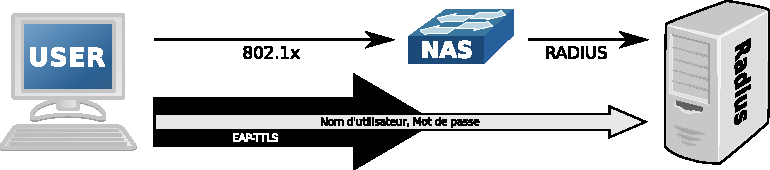
\includegraphics[width=0.7\textwidth]{img/ttls.pdf}
	\end{center}
	\caption{Passage des informations d'authentification en TTLS (double-chiffrement)}
	\label{ttls}
\end{figure}

Dans les trois cas, le serveur dispose d'un  certificat d'autorité qu'il a lui-même généré, en version privée comme publique. Il dispose également d'un certificat d'authentification qu'il a pris soin de s'auto-signer. Les clients ont accès à la version publique de ce dernier. Avec la version publique du certificat d'autorité, ils vérifient la validité du certificat d'authentification publique diffusé par le serveur.

Dans le cas du TLS, le client s'est fait délivrer un couple de certificats privé/publique par le serveur, signés par ce dernier avec le certiticat d'autorité.

En accord avec l'intervenant industriel, nous sommes arrivés à la conclusion qu'il fallait que les authentifications proposent le TLS et le TTLS, pour offrir le choix aux entreprises. Concernant le chiffrement des informations transmises dans le tunnel dans le cas du TTLS, les recherches effectuées aboutissent à la conclusion que la solution mschapv2 est la plus sécurisée. Elle devra donc être utilisée en priorité par les clients.

\subsection{Interface web}
\subsubsection{Langages et environnements de développement}

Le langage PHP a été imposé pour la conception de l'interface web du projet. Le langage a l'avantage d'être suffisamement populaire chez les développeurs, pour assurer sa maintenabilité dans le futur. Il permet une approche de la conception propre et cohérente avec les techniques de développement actuelles, en offrant des performances acceptables y compris pour des serveurs de faible capacité.

Une contrainte sur l'environnement de développement est rapidement venue s'ajouter au langage imposé. Les développeurs de B.H. Consulting ont demandé que l'interface exploite les possibilités du \textit{framework} Bootstrap Twitter. Ce dernier est particulièrement populaire depuis sa récente création par l'entreprise du même nom. Il s'agit d'un composant logiciel pour la partie cliente de l'interface, qui propose une collection très complète de feuilles de style et de dispositions pour créer les vues, afin d'offrir une expérience utilisateur confortable. Une formation rapide de cet outil en interne a dû être effectuée par les membres de l'équipe qui ne l'avaient jamais utilisé auparavant.

Du côté du serveur, l'utilisation d'un \textit{framework} est également conseillée, pour forcer une programmation cohérente et organisée de façon stricte. Il existe plusieurs solutions sur le marché, qui ont conduit à une étude au sein de l'équipe de la meilleure solution à proposer pour la réalisation du projet.

Les plus populaires et puissantes qui ont été retenues sont~:

\begin{itemize}
\item CakePHP
\item CodeIgniter
\item Symfony
\item Yii
\item Zend Framework
\end{itemize}

La conclusion de l'étude a poussé l'équipe à se tourner vers la solution CakePHP. Il s'agit en effet d'un des premiers outils de ce type a être développé pour PHP, basé sur la réalisation de Ruby On Rails, le premier du genre. Il bénéficie donc d'une maturité exemplaire, et dispose d'une communauté rassurante, avec une documentation très complète et très détaillée. La prise en main du logiciel est particulièrement rapide, tout en laissant une grande liberté d'adaptation à tous les usages.

CakePHP n'offre pas toutes les possibilités avancées disponibles avec des solutions plus importantes comme Zend Framework ou Symphony, comme les bibliothèques d'interaction avec d'autres services web tiers (comme Google), mais les fonctionnalités fournies suffisent largement pour le projet et les évolutions qu'il pourrait raisonnablement connaître. Les performances sont particulièrement bonnes en comparaison à ses concurrents plus complets. La solution Yii aurait permis de construire une application qui tient un peu mieux la charge avec des milliers d'utilisateurs, mais l'usage auquel il est destiné pour le projet ne nécessite pas de prendre en compte de telles problématiques.

CakePHP est disponible sous licence libre (MIT). Les patrons de conception populaires sont disponibles, comme le MVC (modèle-vue-contrôleur) qui permet de segmenter l'application de façon propre et efficace. Un fonctionnement en \textit{ActiveRecord} est également disponible, permettant à des classes PHP d'abstraire totalement la liaison entre l'application et la base de données. Les méthodes du modèle intégrent les opérations CRUD (\textit{create}, \textit{read}, \textit{update}, \textit{delete}) permettant de développer rapidement. De nombreuses autres fonctionnalités sont disponibles, comme un dispacheur d'URL, la validation des données, le moteur de patrons facilitant le formatage, la gestion d'un cache, des composants de sécurité et des scripts de génération de code.

La proposition à l'intervenant industriel de cette solution a particulièrement bien été accueillie puisqu'un développeur de l'entreprise utilise cette solution régulièrement, et sera donc à même de maintenir l'interface dans le futur.

\subsubsection{Gestionnaire de bases de données}

Entre les solutions basées sur des implémentations SQL et les nouvelles possibilité de NoSQL (solution alternative qui consiste à ne pas systématiquement privilégier le modèle relationnel), le choix est vaste pour stocker les informations liées à l'interface. Une solution libre étant demandée par l'entreprise, quelques solutions ne sont dors et déjà pas envisageables. 

La meilleure solution pour faire interagir l'interface web avec le serveur Radius étant de réussir à faire fonctionner ce dernier avec une base de données plutôt qu'une collection de fichiers, le choix de la solution s'est fait en ne gardant que les solutions supportées par le fonctionnement de FreeRadius (l'implémentation de Radius choisie auparavant). Cette contrainte élimine toutes les solutions de NoSQL, et réduit le choix aux solutions populaires MySQL et PostgreSQL, éliminant des solutions plus légères comme SQLite qui auraient pu convenir.

PostgreSQL est beaucoup plus puissant que MySQL, mais il est aussi beaucoup plus lourd et plus contraignant à mettre en place. Les possibilités offertes par MySQL et sa simplicité conviennent parfaitement aux exigences du projet.

Le choix de cette solution a été accueilli favorablement par l'intervenant industriel.

\section{Implémentations et méthodologies}
\subsection{Radius}

L'étude des différentes solutions radius aura occupé quelques jours du début du projet, comme en atteste la tâche issue du diagramme de Gantt disponible en figure~\ref{gantt_radius} page~\pageref{gantt_radius}.

\begin{figure}[!h]
	\begin{center}
		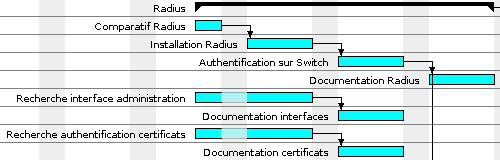
\includegraphics[width=350pt]{img/gantt_radius.png}
	\end{center}
	\caption{Tâche \textit{Radius}}
	\label{gantt_radius}
\end{figure}

Elle a commencé par une recherche documentaire généraliste sur le protocole Radius pour tous les membres de l'équipe, qui a abouti sur l'écriture d'une courte documentation interne. S'en est suivi une recherche plus précise sur les différentes implémentations existantes. Une fois la liste établie, chaque membre a pu s'intéresser plus particulièrement à une solution précise.

La liste des avantages et des inconvénients de chacun a été dressée en réunion, pour conclure sur l'implémentation la plus adaptée à proposer à l'intervenant industriel.

\subsection{Bases de données SQL}

Les recherches concernant le choix de la solution de gestion de bases de données est intimement liée à celui de l'implémentation radius. Ces deux tâches ont donc été exécutées en parallèle, pour trouver une solution globale dans laquelle tous les éléments savent interagir ensemble, tout en étant la plus performante possible.

Le détail de cette tâche issu du diagramme de Gantt est donné en figure~\ref{gantt_sql} page~\pageref{gantt_sql}.

\begin{figure}[!h]
	\begin{center}
		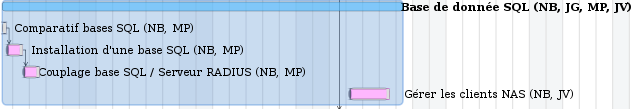
\includegraphics[width=350pt]{img/gantt_sql.png}
	\end{center}
	\caption{Tâche \textit{Bases de données SQL}}
	\label{gantt_sql}
\end{figure}

Après avoir dressé une liste des solutions Open Source les plus populaires, une recherche documentaire a été effecutée sur chacune, pour prendre en compte ses avantages et ses inconvénients. La compatibilité avec les trois principales implémentations Radius retenues a aussi été un critère de choix.

La solution retenue a été installée sur une machine de tests, au côté du Radius gagnant. Une dernière étape a consisté à réussir à lier les deux, pour que l'authentification Radius utilise la base de données SQL.

\subsection{802.1x}

Une dernière étape demeure dans le domaine de la base de données~: gérer les clients NAS, c'est à dire les commutateurs qui auront à utiliser le Radius (et donc indirectement la base de données).

Cette étape s'est faite en parallèle de l'étude du protocole 802.1x, décrite dans la figure~\ref{gantt_dot1x} page~\pageref{gantt_dot1x}.

\begin{figure}[!h]
	\begin{center}
		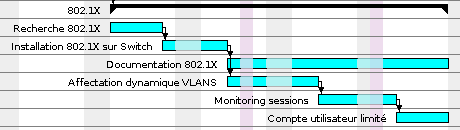
\includegraphics[width=350pt]{img/gantt_dot1x.png}
	\end{center}
	\caption{Tâche \textit{802.1x}}
	\label{gantt_dot1x}
\end{figure}

Celle-ci a logiquement commencé par l'écriture d'une documentation sur le standard, qui a permise à l'équipe de s'auto-former sur la technologie. Après avoir réussi à appliquer nos connaissances sur un commutateur, l'affectation dynamique de réseau virtuel a été testée. Cette première étape valide le coeur-même de notre projet, qui consiste à permettre à une entreprise de graviter le plus simplement possible autour de cette possibilité.

Diverses autres possibilités ont été testées à la main, pour comprendre ce que le protocole permet effectivement de faire, et qui peut nous être utile pour l'implémentation de l'interface web en vue de répondre aux exigences demandées. Ainsi, les tests sur la supervision des sessions ont permis de cerner les différentes possibilités pour identifier le début et la fin d'une session, qui pourra ensuite être affichée graphiquement dans l'interface web. D'autres études comme les limitations pour un utilisateur et les journaux systèmes préparent les futures fonctionnalités de l'interface.

\subsection{Authentifications}

Étape critique du projet, les authentifications au travers du Radius ont été essentielles pour présager du bon fonctionnement de l'ensemble du projet. Elle est décrite dans la figure~\ref{gantt_auth} page~\pageref{gantt_auth}.

\begin{figure}[!h]
	\begin{center}
		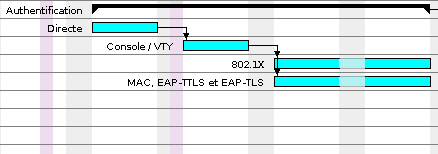
\includegraphics[width=350pt]{img/gantt_auth.png}
	\end{center}
	\caption{Tâche \textit{Authentifications}}
	\label{gantt_auth}
\end{figure}

Les premiers tests ont concerné le Radius directement, et ont abouti sur une authentification de client Radius sur un serveur Radius réussie. La suite aura concerné les commutateurs directement, sur lesquels l'authentification peut se faire aussi directement en Radius (accès à l'interface de configuration du système). Les tests étant concluants, il est possible de contrôler les accès à la configuration d'un commutateur directement grâce à Radius, aussi bien via telnet que le port console.

La suite logique a été de tester directement le protocole 802.1x. L'authentification d'un client sur le Radius au travers du commutateur fonctionnant, il ne reste plus qu'à décliner les solutions pour la certifier.

Jusqu'alors, les authentifications ont été faites en MD5, c'est-à-dire avec uniquement un couple utilisateur/mot de passe, simplement chiffré sur le réseau. Beaucoup de solutions existent, offrant des possibilités très diverses en terme de sécurité et de simplicité d'utilisation. Ces solutions ont été étudiées, documentées, testées et enfin élaguées.

\subsection{Procédure d'installation}

Une fois les différentes tâches concernant le Radius et le SQL terminées, une réinstallation totale du système a été effectuée. Il a ensuite été réinstallé pas-à-pas, grâce aux documentations réalisées durant les tests. Cette étape a été l'occasion de corriger la documentation, et de se confronter à d'autres problèmes mineurs. Cette tâche est décrite en figure~\ref{gantt_finalisation} page~\pageref{gantt_finalisation}.

\begin{figure}[!h]
	\begin{center}
		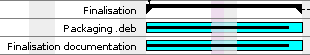
\includegraphics[width=0.5\textwidth]{img/gantt_finalisation.png}
	\end{center}
	\caption{Tâche \textit{Finalisation}}
	\label{gantt_finalisation}
\end{figure}

Un paquet Ubuntu a été réalisé au fur et à mesure de la réinstallation, pour permettre son automatisation. Une dernière réinstallation aura permis de tester son bon fonctionnement. Ce paquet permettra un gain de temps précieux pour l'entreprise, qui aura à le déployer sur toutes les machines d'authentification de ses clients. Différentes questions sont posées durant son installation, pour qu'il s'adapte le plus simplement possible au client.

La réinstallation du système a posé plusieurs fois problème~: les machines mises à disposition ne sont pas parfaitement supportées par Ubuntu et Windows XP. Beaucoup de temps a été perdu pour résoudre les différents problèmes rencontrés.

\subsection{Interface web}

En parallèle de beaucoup des tâches décrites ci-dessus, la prise en main de l'environnement de travail CakePHP a été faite sans aucun lien avec le reste du projet. Ainsi, une seule personne a pris en charge cette étude, en prenant soin de s'auto-former tout en documentant soigneusement ses recherches. Une fois les tâches parallèles terminées, le reste du groupe l'a rejoint, pour une rapide formation sur le sujet. Les sous-tâches sont détaillées dans la figure~\ref{gantt_interface} page~\pageref{gantt_interface}.

\begin{figure}[!h]
	\begin{center}
		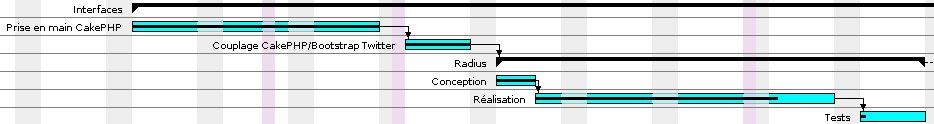
\includegraphics[width=\textwidth]{img/gantt_interface.png}
	\end{center}
	\caption{Tâche \textit{Interface web}}
	\label{gantt_interface}
\end{figure}

L'environnement de travail Bootstrap Twitter étant une prérogative du projet, un temps important a dû être consacré à étudier et tester ses possibles interactions avec CakePHP. Une méthode propre et pratique a été trouvée, permettant au projet d'évoluer rapidement en respectant ses contraintes : un script en langage Javascript a été développé pour modifier les styles générés par CakePHP en style compatible Bootstrap. L'activation de Javascript est donc nécessaire dans le navigateur de l'utilisateur, mais cette contrainte été déjà imposée par CakePHP.
En outre, nous avons décidé d'utiliser FreeRadius en lien avec une base de données MySQL. Il a donc fallu adapter CakePHP pour fonctionner avec le schéma de base de données imposé par FreeRadius. La création des classes (contrôleurs et modèles) se fait facilement en respectant les normes de CakePHP.

Actuellement, l'interface web permet de gérer les utilisateurs de chaque type (Cisco, Identifiant/Mot de passe, adresse MAC, certificats). Les règles correspondantes sont écrites dans la table \emph{radcheck} de la base de données. Il est possible de créer des groupes pour appliquer des règles à un ensemble d'utilisateurs. Une partie de ces règles Radius sont communes aux utilisateurs et aux groupes~: nombre de connexions simultanées, date d'expiration, etc. Enfin, il est possible de gérer les NAS (les commutateurs) qui peuvent se connecter au serveur Radius. Tous ces éléments peuvent être ajoutés, modifiés et supprimés à l'aide de formulaires qui guident l'utilisateur et valident les données insérées.

Des captures de l'interface actuelle sont disponibles en annexe~\ref{captures} page~\pageref{captures}.

\subsection{La suite}

Une vue macro-scopique des tâches à venir est proposée en figure~\ref{gantt_suite} page~\pageref{gantt_suite}. La seconde grande partie du projet démarrera à la suite de la soutenance intermédiaire, avec notamment toute la conception et l'intégration du système de sauvegarde des configurations des équipements actifs. Celui-ci devra permettre de faire des retours arrières en annulant des séries d'actions, tout en proposant des sauvegardes complètes et en surveillant la bonne écriture des modifications sur les équipements.

\begin{figure}[!h]
	\begin{center}
		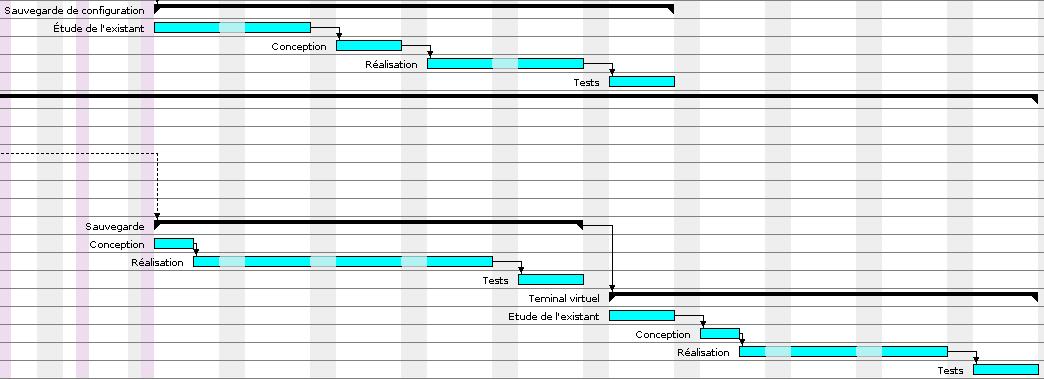
\includegraphics[width=\textwidth]{img/gantt_suite.png}
	\end{center}
	\caption{Vue macro-scopique des tâches à venir}
	\label{gantt_suite}
\end{figure}

Le travail portera donc à la fois sur la recherche des fonctionnalités qui peuvent être utilisées à cet effet sur les équipements, et l'intégration d'un onglet ergonomique dédié à cette tâche dans l'interface. Le développement de cette dernière continue durant cette seconde partie.

\section{Conclusion}

Cette première partie du rapport final étant rédigée pour la soutenance intermédiaire, le temps imparti pour la réalisation du projet est écoulé de moitié. Avec une interface déjà bien avancée et la plupart des recherches abouties, l'équipe démarrera la seconde grande étape dès janvier, respectant ainsi parfaitement les délais prévus dans le planning.

Le matériel attribué au projet dans la salle des projets aura posé beaucoup de problèmes (matériel non-reconnu, disques durs corrompus, crashs inexpliqués, etc.), et aura déjà coûté beaucoup de temps aux membres de l'équipe. Quelques exigences supplémentaires arrivent parfois de la part de l'entreprise (comme la gestion d'utilisateurs d'un pare-feu), venant surcharger le cahier des charges. Nous essayons de faire avec ces contre-temps pour satisfaire l'ensemble des observateurs du projet.

Le système de sauvegardes de la seconde partie impliquant plus de travail sur l'interface web, la première étape de janvier sera de former tous les membres de l'équipe qui n'ont pas encore travaillé dessus.

\newpage
~\vspace{5cm}
\begin{center}
	{\Huge \textbf{Annexes}}
\end{center}
\newpage

\appendix

\section{Note de cadrage}
\label{note-cadrage}

\includepdf[pages=-]{note_de_cadrage.pdf}

\section{Cahier des charges}
\label{cahier-charges}
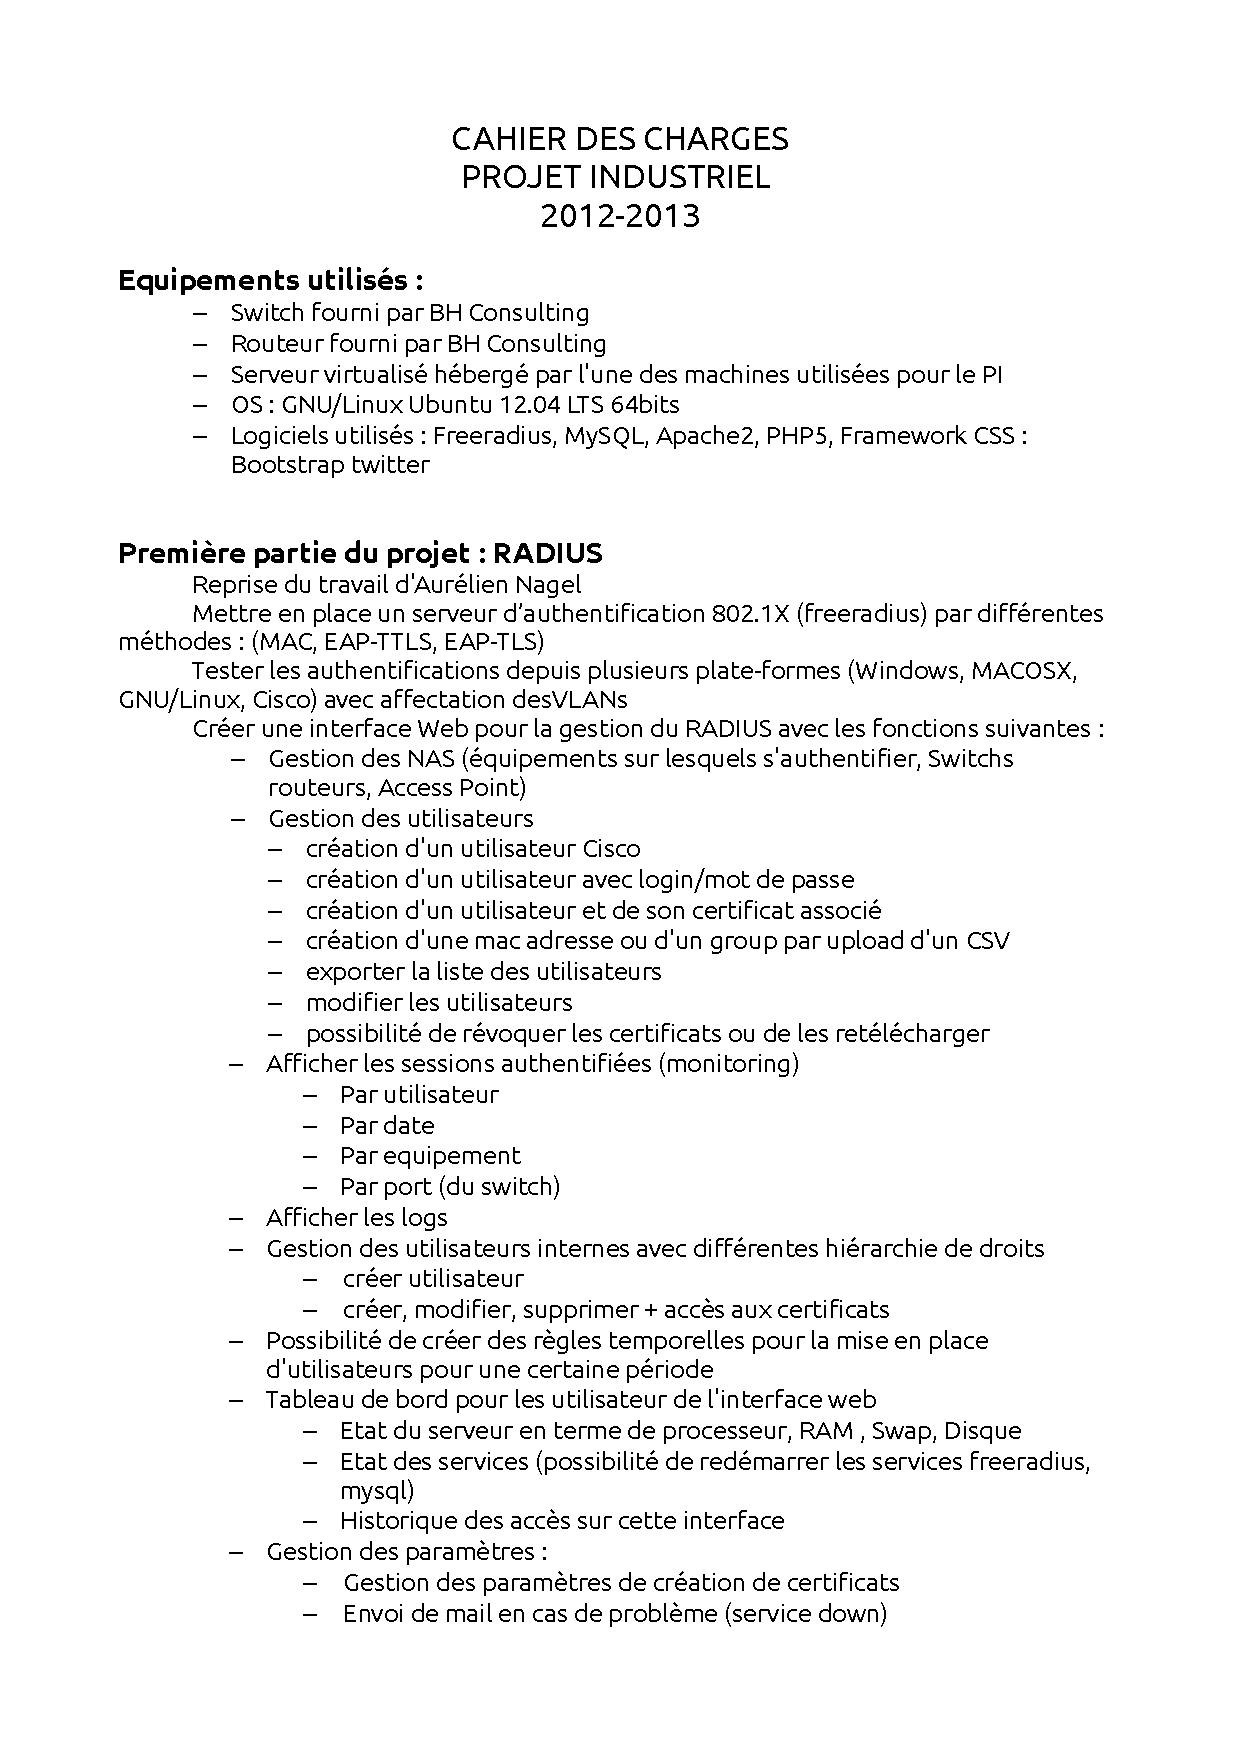
\includepdf[pages=-]{cahier_des_charges.pdf}

\section{Diagramme de Gantt}
\label{gantt}
\begin{center}
	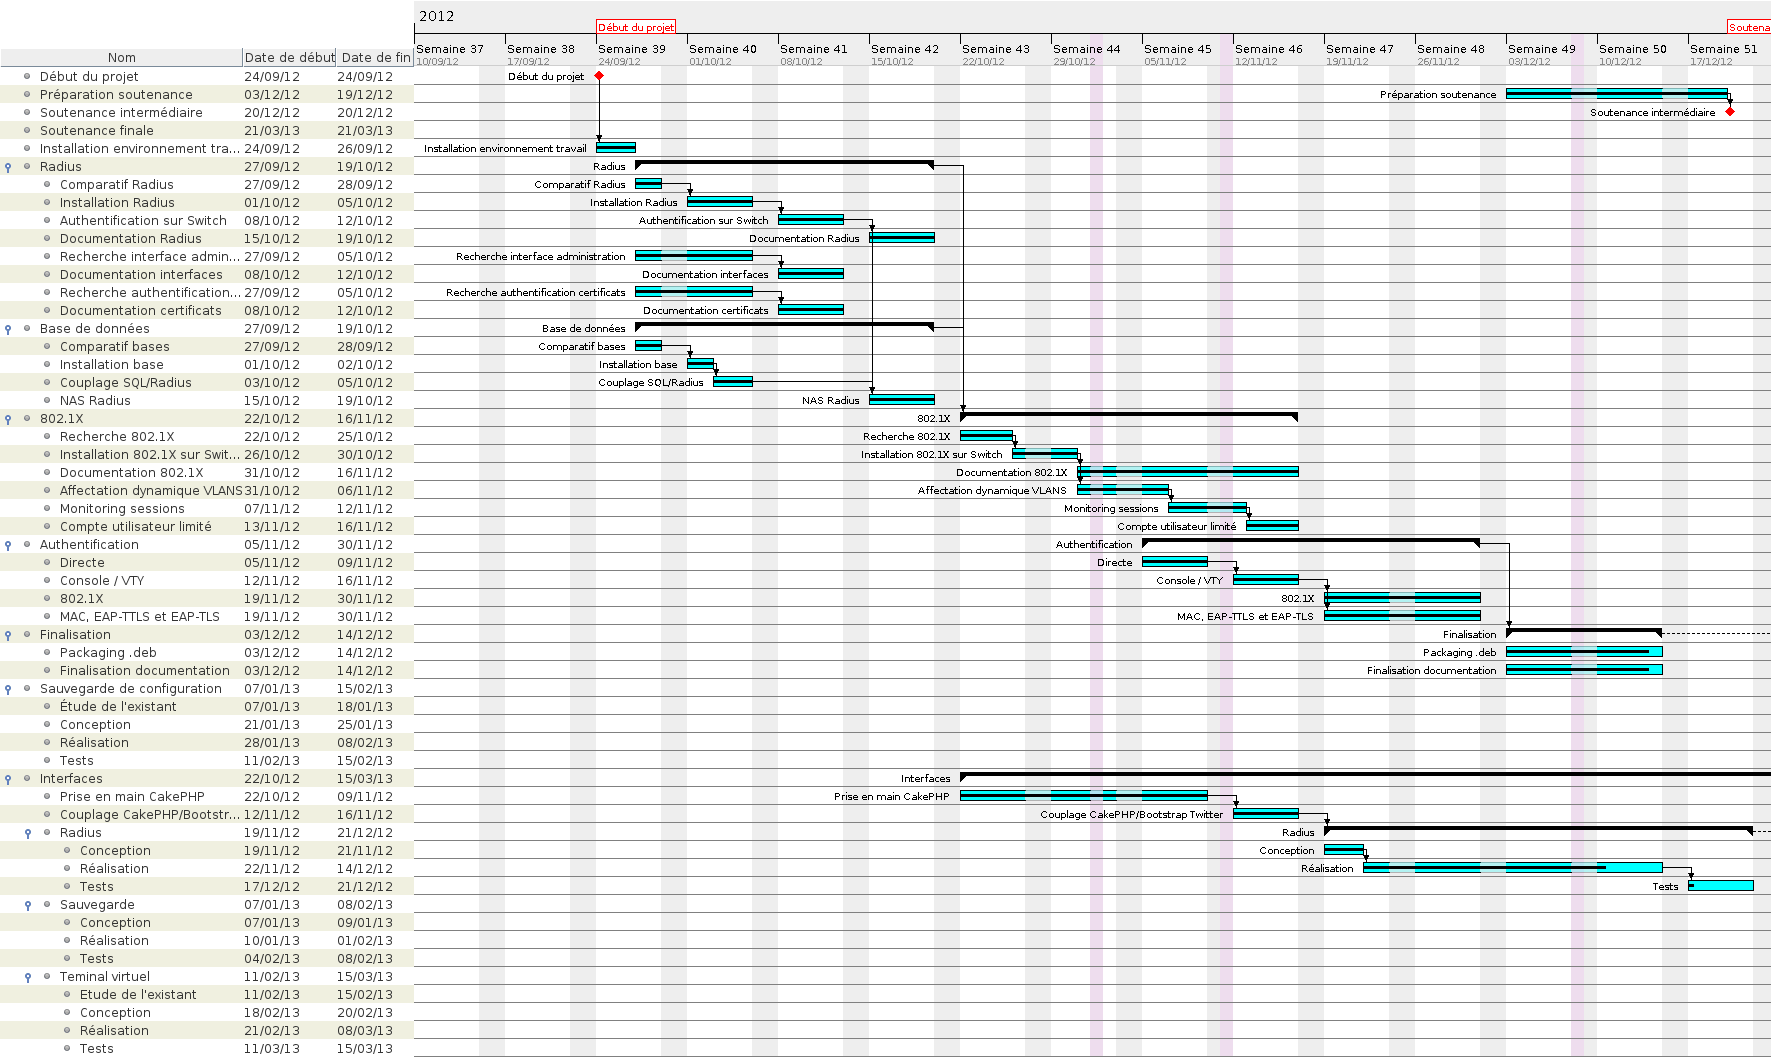
\includegraphics[width=\textwidth]{img/gantt1.png}

	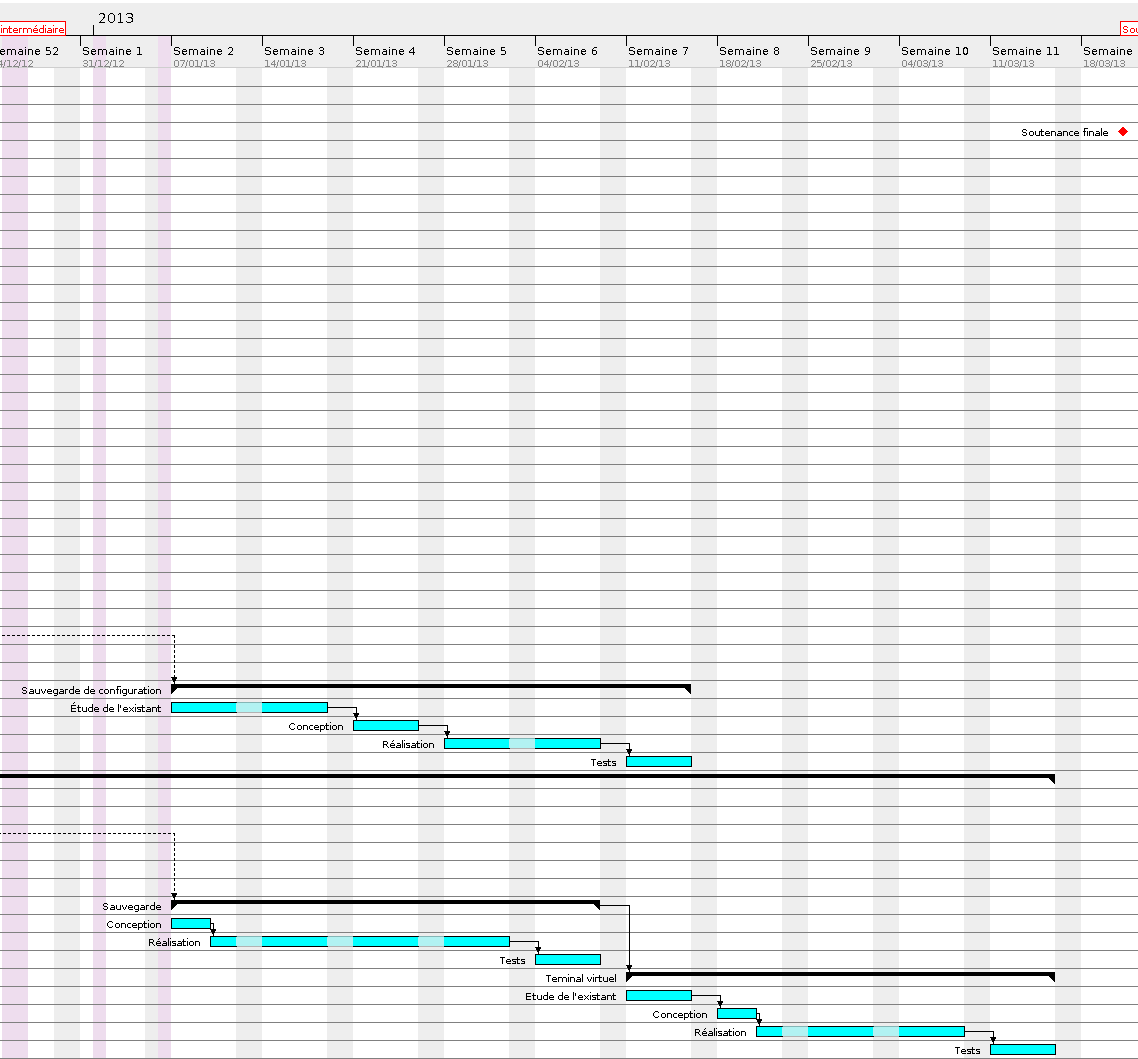
\includegraphics[width=\textwidth]{img/gantt2.png}
\end{center}

\newpage
\section{Captures de l'interface}
\label{captures}

	\begin{figure}[!h]
	\begin{center}
		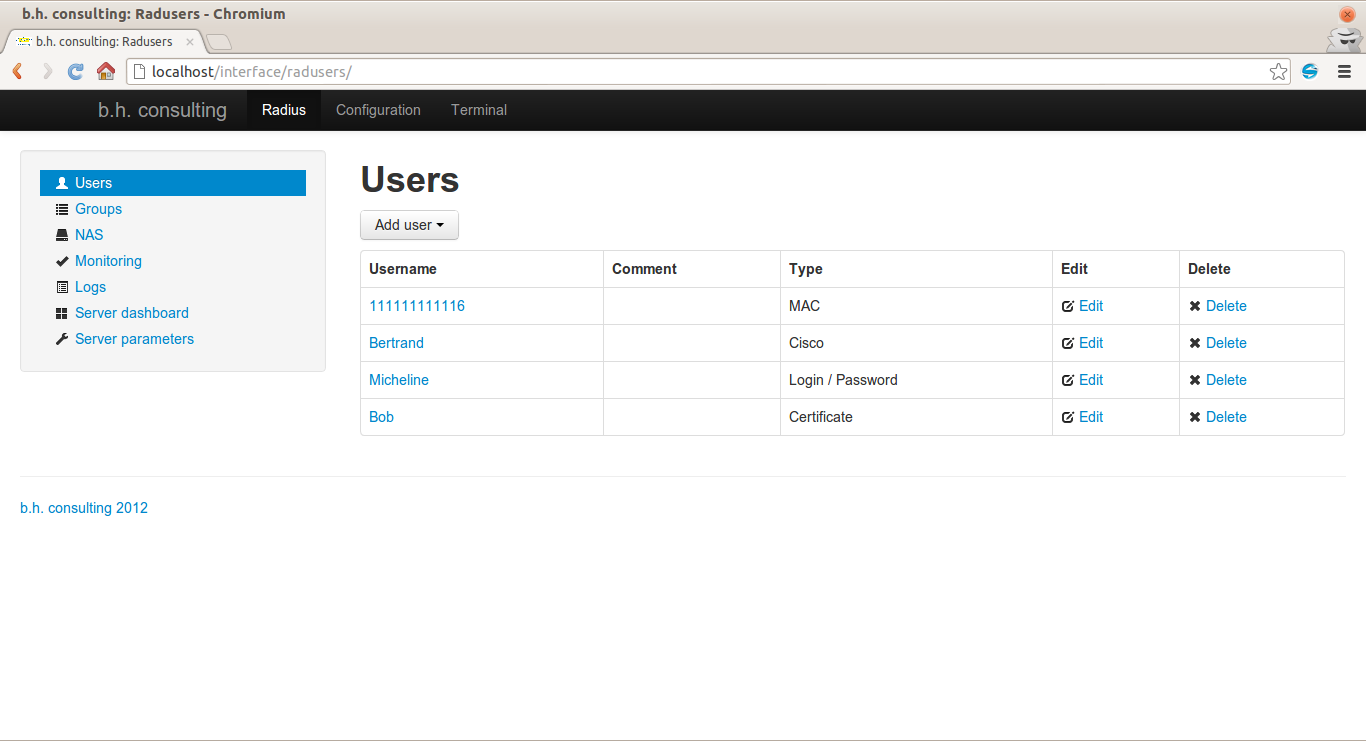
\includegraphics[width=\textwidth]{img/capture2.png}
	\end{center}
	\caption{Liste des utilisateurs Radius}
	\end{figure}

	\begin{figure}[!h]
	\begin{center}
		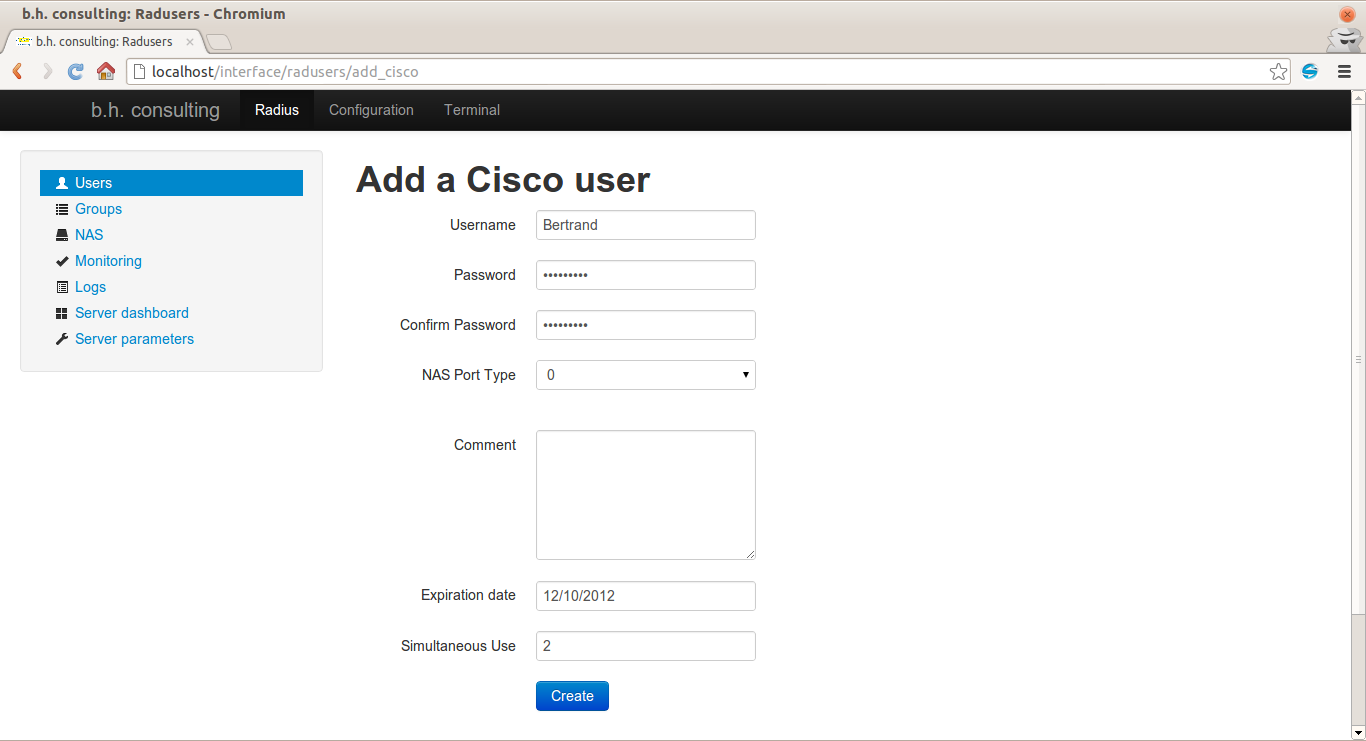
\includegraphics[width=\textwidth]{img/capture1.png}
	\end{center}
	\caption{Formulaire d'ajout d'un utilisateur Cisco}
	\end{figure}

	\begin{figure}[!h]
	\begin{center}
		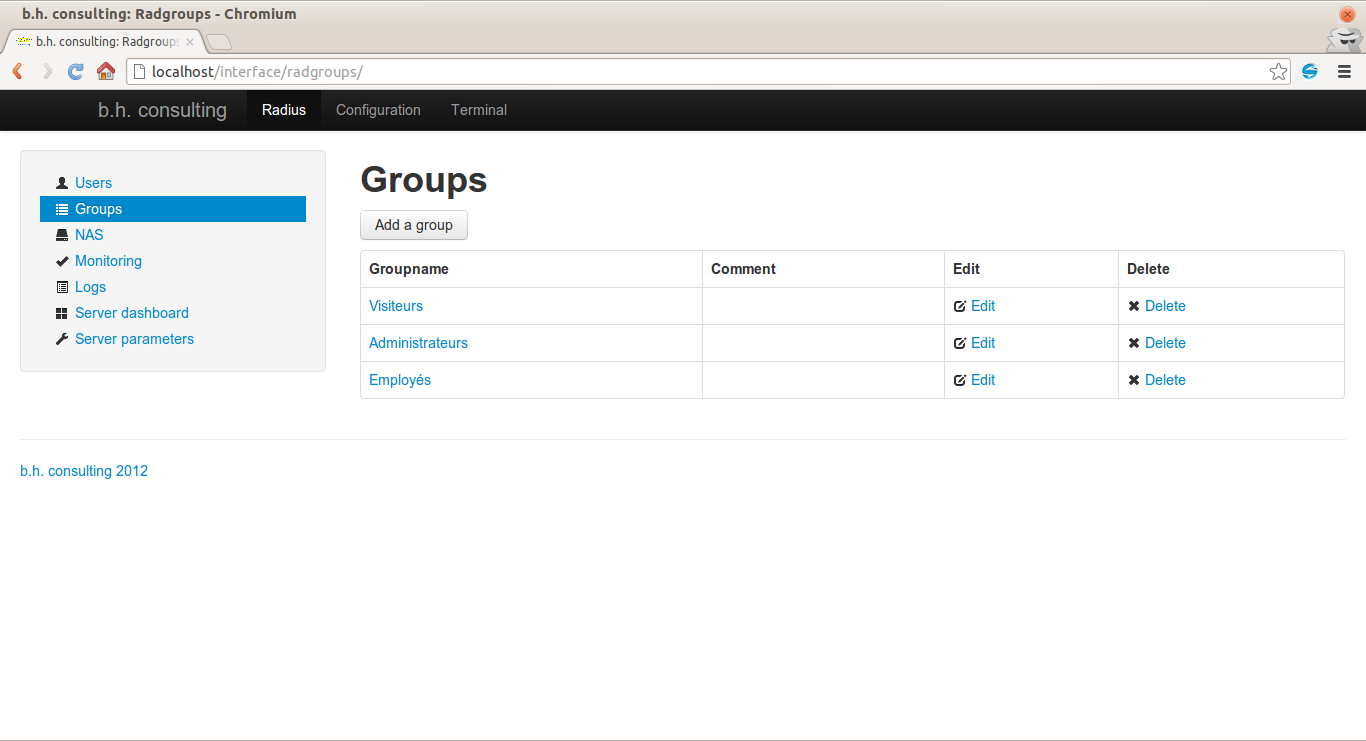
\includegraphics[width=\textwidth]{img/capture3.png}
	\end{center}
	\caption{Liste des groupes Radius}
	\end{figure}

\end{document}
